% !TEX root = ../notes_template.tex

\chapter{테일러 급수와 로랑 급수}

이 장에서는 영역 $D$에 정의된 복소해석함수 $f$는 
$D$의 임의의 점에서 급수 전개가 가능하다는 근본적인 성질을 먼저 공부할 것이다.
다음 그림에서 왼쪽을 참고하라.
\begin{figure*}[h!]
\begin{center}
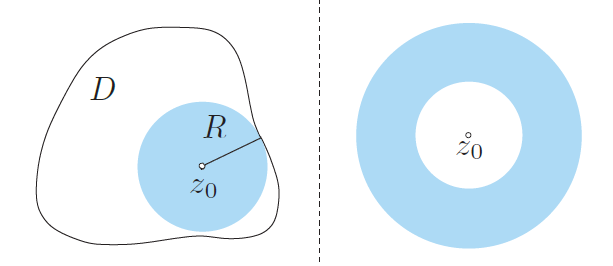
\includegraphics[width=0.5\textwidth]{./SaltChapter/fig-4-0-1}
\end{center}
\end{figure*}
\[
\text{테일러 급수: } \sum_{n=0}^\infty c_n(z-z_0)^n 
\quad
\text{로랑 급수: } \sum_{n\in \mathbb Z} c_n(z-z_0)^n 
\]

즉, 각각의 $z_0 \in D$에 대하여 다음을 만족하는 $R>0$이 존재한다.
\[
f(z) = \sum_{n=0}^\infty c_n(z-z_0)^n, \quad |z-z_0| <R.
\]
역으로,  적당한 $R$에 대하여 $|z-z_0|<R$을 만족하는 두 개 이상의 점에서 급수
\[
\sum_{n=0}^\infty c_n(z-z_0)^n
\]
가 수렴하면 $|z-z_0|<R$에서 복소해석함수이다.
이를 보이는 과정에서 복소해석함수에 대한 근본적인 성질들을 증명할 것이다.
\begin{itemize}
\item[(1)] (일반화된) 코시 적분공식과 코시 부등식
\item[(2)] 해의 분류와 항등정리
\item[(3)] 최대절대값정리
\end{itemize}

이 장의 후반부에서는
급수와 유사하지만 $z-z_0$ 항의 지수를 음의 정수까지 확장한
로랑 급수를 공부할 것이다.
이는 원환(특히 뚫린 원판)에 정의된 복소해석함수를 연구하는데 특히 유용하다,
앞의 그림에서 오른쪽을 참고하라.
끝으로 로랑 급수는 ``특이점''의 분류와 실함수 적분의 계산에도 유용함을 살펴볼 것이다.

\section{급수}

실수열의 경우와 유사하게 주어진
복소수열 $(a_n)_{n\in\mathbb N}$에 대하여
부분합 수열 $(s_n)_{n\in\mathbb N}$을 만들 수 있다.
\begin{align*}
s_1 &:= a_1, \\
s_2 &:= a_1 + a_2, \\
s_3 &:= a_1 + a_2 + a_3, \\
& \vdots
\end{align*}

\begin{salt_definition} \label{def-4-1}
\
\begin{itemize}
\item[(1)] 복소수열 $(s_n)_{n\in\mathbb N}$이 수렴하면
$\sum\limits_{n=1}^\infty a_n := \lim\limits_{n\to\infty} s_n$라 쓰고
급수 $\sum\limits_{n=1}^\infty a_n$이 {\bf 수렴한다}고 정의한다.
\item[(2)] 복소수열 $(s_n)_{n\in\mathbb N}$이 발산하면,
급수 $\sum\limits_{n=1}^\infty a_n$는 {\bf 발산한다}고 정의한다.
\item[(3)] 실급수 $\sum\limits_{n=1}^\infty |a_n|$이 수렴하면,
급수 $\sum\limits_{n=1}^\infty a_n$은 {\bf 절대수렴한다}고 정의한다.
\end{itemize}
\end{salt_definition}

복소수열이 수렴할 필요충분조건은
실수부와 허수부로 만든 수열이 각각 수렴하는 것이라는 
연습문제 \ref{ex-1-25}의 결과로부터,
\[
\sum\limits_{n=1}^\infty a_n\,\text{이 수렴한다. }
\Longleftrightarrow \text{\textcolor{red}{ 실수열} }
\sum\limits_{n=1}^\infty \Re(a_n)\, \text{과 }
\sum\limits_{n=1}^\infty \Im(a_n)\,\text{가 수렴한다.}
\]
따라서  실해석학의 결과를 아용하여 복소수열의 수렴성을 판정할 수 있다.
예를 들면, 다음 결과들을 쉽게 얻을 수 있는데 이는 연습문제로 남긴다.

\begin{salt_exercise}\label{ex-4-1}
$\Sum_{n=1}^\infty a_n$이 수렴하면, $\Lim_{n\to\infty}a_n = 0$임을 보여라.
\end{salt_exercise}

\begin{salt_exercise}\label{ex-4-2}
$\Sum_{n=1}^\infty a_n$이 절대수렴하면, $\Sum_{n=1}^\infty a_n$이 수렴함을 증명하라.
\end{salt_exercise}

\begin{salt_exercise}\label{ex-4-3}
$|z|<1$이면 $\Sum_{n=0}^\infty z^n$이 수렴하고 
$\Sum_{n=0}^\infty z^n = \dfrac1{1-z}$임을 보여라.
\end{salt_exercise}

\begin{salt_exercise}\label{ex-4-4}
$|z|<1$이면 $\Sum_{n=0}^\infty nz^{(n-1)^2}$임을 보여라.
\end{salt_exercise}

\begin{salt_exercise}\label{ex-4-5}
$\Re(s)>0$인 모든 복소수 $s\in \mathbb C$에 대하여
$1^{-s} +  2^{-s} + 3^{-s} + \cdots$가 수렴함을 보여라.
그러면
\[
s \mapsto \zeta(s) := \sum_{n=1}^\infty \dfrac1{n^s}
\]
\end{salt_exercise}
는 반평면 $\Re(s)>1$에서 잘 정의된 함수가 되며, 이를 
{\bf 리만 제타함수}라고 한다.
리만 제타함수와 정수론의 소수이론을 연결한 {\bf 오일러 곱셈공식}에 따르면,
소수를 증가하는 순서대로 나열한
$p_1:=2 < p_2:=3 < p_3:=5 < \cdots$를 무한 소수열로 정의할 때 다음이 성립한다.
\[
\zeta(s) = \lim_{K\to \infty} \prod_{k=1}^K \dfrac1{1-p_k^{-s}},
\quad \Re(s)>1.
\]
버나드 리만(1826-1866)은 제타함수 $\zeta$를 확장하여 $\mathbb C\setminus \{1\}$의 
복소해석함수로 정의할 수 있음을 보였다. 
$\zeta$는 $-2, -4, -6, \ldots$에서 ``자명해(trivial zero)''를 갖지면
다른 해도 존재한다. 리만이 계산한 모든 비자명해(nontrivial zero)는 모두 직선 $\Re(s) = 1/2$위에
있다. 이로부터 리만은 다음과 같이 예측(conjecture)하였는데 이는 여전히 수학계의 유명한 미해결 문제이다.

\begin{salt_conjecture}[리만가설] \label{conj-4-1}
리만 제타함수의 모든 비자명해는 직선 $\Re(s) = 1/2$ 위에 있다.
\end{salt_conjecture}

\section{급수}

\subsection{제곱급수와 수렴영역}

$(c_n)_{n\in\mathbb N}$을 복소수열이라고 하자.
다음과 같은 표현을
\[
\sum_{n=0}^\infty c_nz^n
\]
복소수 변수 $z$의 제곱급수라고 한다 ($(c_n)_{n\in\mathbb N}$을 계수들의 수열로 생각해도 된다).
이제 특정한 값을 급수의  $z$에 대입하는 경우를 생각해볼 수 있다.
그러면 어떤 $z\in\mathbb C$에 대하여 제곱급수가 수렴할 수 있고, 
다른 값에서는 발산할 수도 있다.

\begin{salt_example}\label{example-4-1}
모든 다항식은 유한개의 항에서만 계수가 $0$이 아닌 제곱급수 꼴로 쓸 수 있다.
따라서 다항식은 모든 $z\in\mathbb C$에 대하여 수렴한다.

제곱급수  
\[
\sum_{n=0}^\infty z^n
\]
는 $|z|<1$에서 수렴한다. 
$|z|\ge1$에서 급수는 발산한다 (왜냐하면 $\Lim_{n\to\infty} z^n = 0$이 성립하지 않으므로).
\hfill$\diamondsuit$
\end{salt_example}

근본적인 질문으로 
\begin{center}
어떤 $z\in\mathbb C$에 대하여  급수 $\sum_{n=0}^\infty c_nz^n$가 수렴하는가?
\end{center}

이 문제에 대한 답은 다음 정리에서 얻을 수 있다.

\begin{salt_theorem} \label{thm-4-1}
급수 $\Sum_{n=0}^\infty c_nz^n$에 대하여
다음 두 가지 중 정확히 하나만 성립한다.
\begin{itemize}
\item[(1)] 모든 $z\in\mathbb C$에 대하여 절대수렴하거나
\item[(2)] 음이 아닌 실수 $R$이 유일하게 존재하여 다음을 만족한다.
\begin{itemize}
\item[(a)] $|z|<R$인 모든 $z\in\mathbb C$에 대하여 $\Sum_{n=0}^\infty c_nz^n$이 절대수렴하고,
\item[(b)] $|z|>R$인 모든 $z\in\mathbb C$에 대하여 $\Sum_{n=0}^\infty c_nz^n$는 발산한다.
\end{itemize}
\end{itemize}
\end{salt_theorem}

위 정리에서 유일한 $R>0$을 급수의 수렴반경이라 부른다.
급수가 모든 $z\in\mathbb C$에 대하여 수렴하면
무한대의 수렴반경을 가지며 ``$R=\infty$''라 쓴다.

\begin{figure}[h!]
\begin{center}
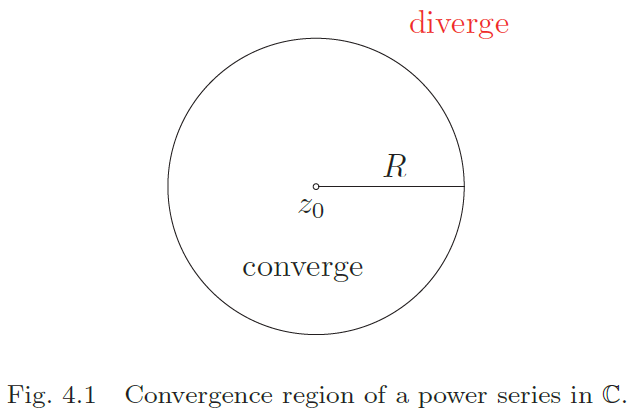
\includegraphics[width=0.5\textwidth]{./SaltChapter/fig-4-1}
\end{center}
\caption{$\mathbb C$에 정의된 제곱급수의 수렴영역}
\label{fig-4-1}
\end{figure}

원 $|z|=R$에서는 어떻게 될까?
복소 제곱급수는 $|z|=R$로 주어진 경계의 모든 점에서 발산하거나,
어떤 점에서는 발산하고 어떤 점에서는 수렴하거나,
아니면 경계의 모든 점에서 수렴할 수도 있다.
경계위의 각 점에 대하여 어떻게 되는지 답을 구하는 일반적인 방법은 없다.
특정한 제곱급수가 주어지면 그 특성에 따라 찾아 직접 확인해야 한다,

{\bf 증명} (정리 \ref{thm-4-1})

\[
S:= \left\{ y\in [0,\infty) \,:\,
\exists z\in \mathbb C, y=|z| \text{ 이고 } \Sum_{n=0}^\infty c_nz^n \text{이 수렴한다.}
\right\}
\]
라 정의하자.





